\documentclass[a4paper,11pt,twoside]{memoir}
\chapterstyle{veelo}

\usepackage{TUINFDA}

\usepackage{url}
\usepackage{hyperref}					% links in pdf
\usepackage{cleveref}
\usepackage{graphicx}            			% Figures
\usepackage{verbatim}            			% Code-Environment
\usepackage[lined,linesnumbered,algochapter]{algorithm2e} % Algorithm-Environment

\usepackage{pgf}					
\usepackage{tikz}					% tikz graphics
\usetikzlibrary{arrows,automata}

\usepackage{ngerman}
\usepackage[ngerman]{babel}
\usepackage{bibgerm,cite}       % Deutsche Bezeichnungen, Automatisches Zusammenfassen von Literaturstellen
\usepackage[ngerman]{varioref}  % Querverweise
% to use the german charset include cp850 for MS-DOS, ansinew for Windows and latin1 for Linux.
% \usepackage[latin1]{inputenc}

\thesistitle{Kosteneffizientes Ressourcenmanagement in verteilten Cloud Datenzentren}{Cost aware resource management in distributed cloud data centers}
\thesissubtitle{} % optional
\thesisdate{28.07.2015}

% all titles and designations have to be gender-related!
\thesisdegree{Diplom-Ingenieur}{Master of Science}
\thesiscurriculum{Informatik}{Computer Science} % your study
\thesisverfassung{Verfasser} % Verfasser
\thesisauthor{Andreas Egger} % your name
\thesisauthoraddress{Ospelgasse 35/3, 1200 Wien} % your address
\thesismatrikelno{0626885} % your registration number

\thesisbetreins{Priv.-Doz. Dr. Ivona Brandić}
\thesisbetrzwei{MSc. Dražen Lučanin}
\thesisbetrdrei{} % optional

% define page numbering styles
\makepagestyle{numberCorner}
\makeevenfoot{numberCorner}{\thepage}{}{}
\makeoddfoot{numberCorner}{}{}{\thepage}

% define custom macros for specific formats or names
\newcommand{\uml}[1]{\texttt{#1}}
\newcommand{\cd}{\textsf{Class Diagram}}

\begin{document}

\captionnamefont{\bfseries}

%%%%%%%%%%%%%%%%%%%%%%%%%%%%%%%%%%%%%%%%%
%%%   FRONTMATTER    %%%%%%%%%%%%%%%%%%%%
%%%%%%%%%%%%%%%%%%%%%%%%%%%%%%%%%%%%%%%%%
\frontmatter
\pagenumbering{roman}

%%%%%%%%%%%%%%%%%%%%%%%%%%%%%%%%%%%%%%%%%
%%%   TITLEPAGES    %%%%%%%%%%%%%%%%%%%%%
%%%%%%%%%%%%%%%%%%%%%%%%%%%%%%%%%%%%%%%%%

% the german title page is required as first page
% $Id: titlepage.tex 1752 2010-03-20 11:07:02Z tkren $
%
% TU Wien - Faculty of Informatics
% thesis titlepage
%
% This titlepage is using the geometry package, see
% <http://www.ctan.org/macros/latex/contrib/geometry/geometry.pdf>
%
% For questions and comments send an email to
% Thomas Krennwallner <tkren@kr.tuwien.ac.at>
% or to Petra Brosch <brosch@big.tuwien.ac.at>
%

\selectlanguage{ngerman}

% setup page dimensions for titlepage
\newgeometry{left=2.4cm,right=2.4cm,bottom=2.5cm,top=2cm}

% force baselineskip and parindent
\newlength{\tmpbaselineskip}
\setlength{\tmpbaselineskip}{\baselineskip}
\setlength{\baselineskip}{13.6pt}
\newlength{\tmpparindent}
\setlength{\tmpparindent}{\parindent}
\setlength{\parindent}{17pt}

% first titlepage
\thispagestyle{tuinftitlepage}

%
% Kludge: for each titlepage set \pagenumbering to a different
% style. This is used to fix a problem with hyperref, because there
% are multiple "page 1" and hyperref hates that
%
\pagenumbering{Alph}

\begin{center}
{\ \vspace{3.4cm}}

\begin{minipage}[t][2.8cm][s]{\textwidth}%
\centering
\thesistitlefontHUGE\sffamily\bfseries\tuinfthesistitle\\
\bigskip
{\thesistitlefonthuge\sffamily\bfseries\tuinfthesissubtitle}
\end{minipage}

\vspace{1.3cm}

{\thesistitlefontLARGE\sffamily \tuinfthesistype}

\vspace{6mm}

{\thesistitlefontlarge\sffamily zur Erlangung des akademischen Grades}

\vspace{6mm}

{\thesistitlefontLARGE\sffamily\bfseries \tuinfthesisdegree}

\vspace{6mm}

{\thesistitlefontlarge\sffamily im Rahmen des Studiums}

\vspace{6mm}

{\thesistitlefontLarge\sffamily\bfseries \tuinfthesiscurriculum}

\vspace{6.5mm}

{\thesistitlefontlarge\sffamily eingereicht von}

\vspace{6mm}

{\thesistitlefontLarge\sffamily\bfseries \tuinfthesisauthor}

\vspace{1.5mm}

{\thesistitlefontlarge\sffamily Matrikelnummer \tuinfthesismatrikelno} 

\vspace{1.4cm}

\vspace{0pt}\raggedright\thesistitlefontnormalsize\sffamily
\begin{minipage}[t][1.6cm][t]{\textwidth}%
  %
  an der

  Fakult\"{a}t f\"{u}r Informatik der Technischen Universit\"{a}t Wien
\end{minipage}

\begin{minipage}[t][4cm][t]{\textwidth}%
  \vspace{0pt}\raggedright\thesistitlefontnormalsize\sffamily
  %
  \begin{tabbing}%
	    \hspace{19mm} \= \hspace{66mm} \kill
	    \tuinfthesisbetreuung: \> \tuinfthesisbetreins\\
	    Mitwirkung: \> \tuinfthesisbetrzwei\\
	                \> \tuinfthesisbetrdrei
  \end{tabbing}
\end{minipage}

\begin{minipage}[t][1.5cm][t]{\textwidth}%
  \vspace{0pt}\sffamily\thesistitlefontnormalsize
  \begin{tabbing}%
    \hspace{45mm} \= \hspace{63mm} \= \hspace{51mm} \kill
    Wien, \tuinfthesisdate \> {\raggedright\rule{51mm}{0.5pt}} \> {\raggedright\rule{51mm}{0.5pt}} \\
    \> \begin{minipage}[t][0.5cm][t]{51mm}\centering (Unterschrift \tuinfthesisverfassung)\end{minipage}
    \> \begin{minipage}[t][0.5cm][t]{51mm}\centering (Unterschrift \tuinfthesisbetreuung)\end{minipage}
    \end{tabbing}
\end{minipage}

\end{center}

% we want an empty page right after first titlepage
\pagestyle{empty}
\cleardoublepage

% we're done with the titlepages, proceed with default pagenumbering
\pagenumbering{roman}

% restore baselineskip
\setlength{\baselineskip}{\tmpbaselineskip}
\setlength{\parindent}{\tmpparindent}

% back to normal geometry
\restoregeometry

\selectlanguage{english}

%%% Local Variables:
%%% TeX-PDF-mode: t
%%% TeX-debug-bad-boxes: t
%%% TeX-parse-self: t
%%% TeX-auto-save: t
%%% reftex-plug-into-AUCTeX: t
%%% End:


% an english translation may follow
% $Id: titlepage.tex 1752 2010-03-20 11:07:02Z tkren $
%
% TU Wien - Faculty of Informatics
% thesis titlepage
%
% This titlepage is using the geometry package, see
% <http://www.ctan.org/macros/latex/contrib/geometry/geometry.pdf>
%
% For questions and comments send an email to
% Thomas Krennwallner <tkren@kr.tuwien.ac.at>
% or to Petra Brosch <brosch@big.tuwien.ac.at>
%

% setup page dimensions for titlepage
\newgeometry{left=2.4cm,right=2.4cm,bottom=2.5cm,top=2cm}

% force baselineskip and parindent
%\newlength{\tmpbaselineskip}
%\setlength{\tmpbaselineskip}{\baselineskip}
%\setlength{\baselineskip}{13.6pt}
%\newlength{\tmpparindent}
%\setlength{\tmpparindent}{\parindent}
%\setlength{\parindent}{17pt}

% first titlepage
\thispagestyle{tuinftitlepage}

%
% Kludge: for each titlepage set \pagenumbering to a different
% style. This is used to fix a problem with hyperref, because there
% are multiple "page 1" and hyperref hates that
%
\pagenumbering{Roman}

\begin{center}
{\ \vspace{3.4cm}}

\begin{minipage}[t][2.8cm][s]{\textwidth}%
\centering
\thesistitlefontHUGE\sffamily\bfseries\tuinfthesistitle\\
\bigskip
{\thesistitlefonthuge\sffamily\bfseries\tuinfthesissubtitle}
\end{minipage}

\vspace{1.3cm}

{\thesistitlefontLARGE\sffamily \tuinfthesistypeen}

\vspace{6mm}

{\thesistitlefontlarge\sffamily submitted in partial fulfillment of the requirements for the degree of}

\vspace{6mm}

{\thesistitlefontLARGE\sffamily\bfseries \tuinfthesisdegreeen}

\vspace{6mm}

{\thesistitlefontlarge\sffamily in}

\vspace{6mm}

{\thesistitlefontLarge\sffamily\bfseries \tuinfthesiscurriculumen}

\vspace{6.5mm}

{\thesistitlefontlarge\sffamily by}

\vspace{6mm}

{\thesistitlefontLarge\sffamily\bfseries \tuinfthesisauthor}

\vspace{1.5mm}

{\thesistitlefontlarge\sffamily Registration Number \tuinfthesismatrikelno} 

\vspace{1.4cm}

\begin{minipage}[t][1.6cm][t]{\textwidth}%
  \vspace{0pt}\raggedright\thesistitlefontnormalsize\sffamily
  %
  to the Faculty of Informatics 

  at the Vienna University of Technology
\end{minipage}

\vspace{0pt}\raggedright\thesistitlefontnormalsize\sffamily
\begin{minipage}[t][4cm][t]{\textwidth}%
  \begin{tabbing}%
	    \hspace{19mm} \= \hspace{66mm} \kill
	    Advisor: \> \tuinfthesisbetreins\\
	    Assistance: \> \tuinfthesisbetrzwei\\
	                \> \tuinfthesisbetrdrei
     \end{tabbing}
\end{minipage}

\begin{minipage}[t][1.5cm][t]{\textwidth}%
  \vspace{0pt}\sffamily\thesistitlefontnormalsize
  \begin{tabbing}%
    \hspace{45mm} \= \hspace{63mm} \= \hspace{51mm} \kill
    Vienna, \tuinfthesisdate \> {\raggedright\rule{51mm}{0.5pt}} \> {\raggedright\rule{51mm}{0.5pt}} \\
    \> \begin{minipage}[t][0.5cm][t]{51mm}\centering (Signature of Author)\end{minipage}
    \> \begin{minipage}[t][0.5cm][t]{51mm}\centering (Signature of Advisor)\end{minipage}
    \end{tabbing}
\end{minipage}

\end{center}

% we want an empty page right after first titlepage
\pagestyle{empty}
\cleardoublepage

% we're done with the titlepages, proceed with default pagenumbering
\pagenumbering{roman}

% restore baselineskip
\setlength{\baselineskip}{\tmpbaselineskip}
\setlength{\parindent}{\tmpparindent}

% back to normal geometry
\restoregeometry


%%% Local Variables:
%%% TeX-PDF-mode: t
%%% TeX-debug-bad-boxes: t
%%% TeX-parse-self: t
%%% TeX-auto-save: t
%%% reftex-plug-into-AUCTeX: t
%%% End:
 % optional

%%%%%%%%%%%%%%%%%%%%%%%%%%%%%%%%%%%%%%%%%
%%%   ERKLAERUNG DER SELBSTAENDIGKEIT   %
%%%%%%%%%%%%%%%%%%%%%%%%%%%%%%%%%%%%%%%%%
\cleardoublepage
\selectlanguage{ngerman}
\chapter*{Erklärung zur Verfassung der Arbeit}

\tuinfthesisauthor\\
\tuinfthesisauthoraddress

\vspace*{1.2cm}

Hiermit erkläre ich, dass ich diese Arbeit selbständig verfasst habe, 
dass ich die verwendeten Quellen und Hilfsmittel vollständig angegeben 
habe und dass ich die Stellen der Arbeit - einschließlich Tabellen, 
Karten und Abbildungen -, die anderen Werken oder dem Internet im 
Wortlaut oder dem Sinn nach entnommen sind, auf jeden Fall unter Angabe 
der Quelle als Entlehnung kenntlich gemacht habe.\\

\vspace*{2cm}
\begin{tabbing}%
    \hspace{58mm} \= \hspace{28mm} \= \hspace{58mm} \kill
    {\raggedright\rule{58mm}{0.5pt}} \> \> {\raggedright\rule{58mm}{0.5pt}} \\
    \begin{minipage}[t][0.5cm][t]{58mm}
	\vspace{0pt}\sffamily\thesistitlefontnormalsize
	\centering (Ort, Datum)
    \end{minipage}
    \> \>
    \begin{minipage}[t][0.5cm][t]{58mm}
	\vspace{0pt}\sffamily\thesistitlefontnormalsize
	\centering (Unterschrift \tuinfthesisverfassung)
    \end{minipage}
\end{tabbing}


\selectlanguage{english}

%%%%%%%%%%%%%%%%%%%%%%%%%%%%%%%%%%%%%%%%%
%%%   ACKNOWLEDGEMENTS    %%%%%%%%%%%%%%%
%%%%%%%%%%%%%%%%%%%%%%%%%%%%%%%%%%%%%%%%%

% optional acknowledgements may be included in german or in english
%\chapter*{Danksagung}

Hier fügen Sie optional eine Danksagung ein.
 		% optional
\chapter*{Acknowledgements}

Optional acknowledgements may be inserted here.	% optional

%%%%%%%%%%%%%%%%%%%%%%%%%%%%%%%%%%%%%%%%%
%%%   ABSTARCT    %%%%%%%%%%%%%%%%%%%%%%%
%%%%%%%%%%%%%%%%%%%%%%%%%%%%%%%%%%%%%%%%%

\chapter*{Abstract}

Cloud computing services experienced increasing popularity over the recent years which caused the power demand of data centers to increase significantly. 
As energy costs represent a significant part of the total cost of data centers energy cost reductions in cloud computing environments play an important role for cloud providers to remain competitive and provide affordable cloud services. This thesis introduces a cloud framework to evaluate energy cost reductions in multi electricity market environments. It is shown that substantial cost savings are possible using intelligent resource scheduling algorithms with integration of energy price forecasts. 

This thesis consists of two parts. In the first part different forecasting models are evaluated to assess the performance of the models for energy price time series of different energy markets. A forecast simulation framework is introduced capable of dynamically managing energy price data from different power markets and generating forecasts based on that data. The framework incorporates methods for automatic model generation and evaluation as a basis for extended forecast simulations. 
A large scale forecast evaluation is conducted to gain insights into model accuracy across a wide range of energy price data. Different training periods, forecast horizons and energy price datasets lead to a comprehensive evaluation of the forecasting models. 

The second part is dedicated to large scale cloud simulations comprising different cloud schedulers and scenarios. An existing cloud simulation framework has been extended to perform simulations across a wide range of energy price data where different scheduling mechanisms have been introduced. 
A utility function has been defined for sophisticated evaluation of different criteria to decide on the best suitable VMs to migrate at any point in time. Criteria involve probability of SLA penalties and maximum cost benefits to appropriately handle the tradeoff between minimizing costs and providing an adequate level of quality of service. 

Results show that significant cost savings are possible with schedulers incorporating different criteria and energy price forecasts revealing promising results. Based on the defined cloud settings it illustrates the applicability of the proposed approach to real world scenarios of geo-distributed data centers connected to energy markets. 



\cleardoublepage
\selectlanguage{ngerman}
\chapter*{Kurzfassung}

Hier fügen Sie die Kurzfassung auf Deutsch gemäß den Vorgaben der Fakultät ein.

\selectlanguage{english}

%%%%%%%%%%%%%%%%%%%%%%%%%%%%%%%%%%%%%%%%%
%%%   CONTENTS    %%%%%%%%%%%%%%%%%%%%%%%
%%%%%%%%%%%%%%%%%%%%%%%%%%%%%%%%%%%%%%%%%
% uncomment to set document language to german (results in "Inhaltsverzeichnis", "Kapitel", "Abbildung", etc. instead of "Contents", "Chapter", and "Figure"), otherwise the document's language is english
%\selectlanguage{ngerman}

\setcounter{tocdepth}{1}

\cleardoublepage
\pagestyle{numberCorner}
\tableofcontents*

%%%%%%%%%%%%%%%%%%%%%%%%%%%%%%%%%%%%%%%%%
%%%   MAINMATTER    %%%%%%%%%%%%%%%%%%%%%
%%%%%%%%%%%%%%%%%%%%%%%%%%%%%%%%%%%%%%%%%

\mainmatter
\pagenumbering{arabic}
\pagestyle{numberCorner}


%%%%%%%%%%%%%%%%%%%%%%%%%%%%%%%%%%%%%%%%%
% 		 	Definition of remarks 					%
%																				%
% [c] - insert citation									%
% [r] - remove/replace prev. statement 	%
% [g] - insert graphic									%
%																				%
%%%%%%%%%%%%%%%%%%%%%%%%%%%%%%%%%%%%%%%%%


%%%%%%%%%%%%%%%%%%%%%%%%%%%%%%%%%%%%%%%%%
\chapter{Introduction}
\label{ch:intro}
%%%%%%%%%%%%%%%%%%%%%%%%%%%%%%%%%%%%%%%%%



\section{Motivation}

In times of cloud computing where computer resources are expected to be readily available from anywhere \cite{buyya2009cloud} and with an ever growing global network of interconnected devices cloud providers need to cope with increasing energy consumption in data centers as requests need to be handled at a rapid pace. 
As energy consumption is directly mapped to energy costs, cloud providers aim to reduce power consumption and thus electricity costs within data centers. 

Studies show that electricity costs for cloud systems comprising several large scale data centers is in the range of tens of millions of dollars per year \cite{qureshi2009cutting}. Energy consumption, related energy costs and high energy prices may slow down or hinder advancements in cloud computing. Thus, cloud providers must ensure that delivering their services remains profitable. Lower energy costs increase the competitive ability of cloud providers and bigger investments are possible. Likewise customers may benefit from more affordable cloud services. 

Energy cost reductions can be addressed by utilizing one of two different approaches. One common approach is to increase energy efficiency in data centers to reduce energy consumption and therefore energy related costs as well [c]. This is done i.e.~by utilizing more energy efficient hardware, implementing an energy efficient cooling system, virtualization of servers or energy aware load distribution policies. It additionally aims at minimizing the Power Usage Effectiveness (PUE) of data centers which describes the ratio of the total amount of power consumed to the power consumed solely by IT equipment\footnote{http://www.itwissen.info/definition/lexikon/power-usage-effectivness-PUE.html} [r]. Despite the importance of increasing energy efficiency to reduce costs and environmental load this approach is limited as energy efficiency may not be improved beyond a critical point where investments in energy efficiency measures do not further reduce overall energy expenses [g]. 
%Thus the expenses of auxiliary systems should be reduced to a minimum to spend less on electricity. 
%Two common approaches address the reduction of energy costs in data centers. 

The second approach is directed at intelligent scheduling mechanisms based on dynamically changing energy prices. In wholesale power markets energy prices commonly change at an hourly basis with factors up to 10 from one hour to the next [c]. Electricity price behavior of power markets may differ significantly with possibly involved seasonality patterns where different time zones lead to substantial locational price differences. These characteristics of locational and temporal varying energy prices may be exploited by intelligent scheduling algorithms and cost aware resource management routines that place requests at facilities currently exhibiting low energy prices. In addition the current energy price time series at any location and time stamp is observed and resources may be migrated to data centers that currently operate below peak load and facing low energy prices. %where energy prices are currently cheaper. 

The focus of this thesis is to go beyond intelligent scheduling of resources %to fit the current distribution of energy prices 
by integrating sophisticated forecasting methods that predict price time series behaviors into the near future. This measure is expected to further optimize resource distribution across data centers by comparing and analyzing current and predicted energy price time series to find the best fit of resources in the near future which should result in the maximum possible energy cost reduction.

%The goal of this thesis is to reduce energy related costs of interconnected data centers with respect to changing energy prices in wholesale power markets. 
%The proposed approach is to optimize load placement and migration between data centers considering time and location based energy prices. 
%In addition to placing resources at locations currently facing low energy prices the resources or virtual machines are migrated to sites where low energy prices are \emph{expected} in the near future. 

%The scenario includes data centers located in different countries where different energy markets and prices apply. Thus constellations may arise where it is profitable to migrate a certain amount of resources from a data center facing high energy prices to a data center where energy prices are low at the current point in time or in the near future. 

\section{Problem Statement}

Energy prices are traded and change hourly within the energy markets, so investigations need to be made in order to make qualified statements about the estimated energy price at some point in time in the near future.
This is done by analyzing historical price data and building models for accurate energy price forecasting. Energy prices belonging to different energy markets are estimated for various time ranges into the future. Based upon the results it is decided how many resources may be migrated currently or in the future in order to obtain the maximum possible energy cost reduction. 
However, forecasting errors represented by the difference between estimated and real energy prices increase with the length of the estimation window which has to be taken into account when determining the length of the forecasting window. 

Since energy prices change dynamically a flexible approach of moving data center resources to more cost-effective locations is needed. This work is based on the scenario of a company running data centers distributed across several countries. Depending on the current and estimated energy price for a certain region resources may be relocated to other data centers located at more cost-effective regions.

The key technology to implement the relocation of data center resources is virtual machine (VM) migration \cite{nelson2009virtual}. All data and services are located on servers and belong to specific virtual machines within a data center. Since a server may host several VMs that operate completely independent from each other, they can be relocated (migrated) to other servers, possibly over networks without affecting VMs running on the same server. VM migration may be applied across large geographical distances (geo migrations) by leveraging connections via the internet. It is also possible to do live migrations on a large scale without noticeable service interruption \cite{celesti2010improving}. 

Various load policies exist to optimize the load factor and distribution of tasks within data centers \cite{buyya2010energy}. A workload manager has to make sure that there are still servers having enough resources and no service level agreement (SLA) is violated on the assignment of a new job. 
In contrast, this work aims to optimize workload distribution among geographically distributed data centers with a focus on the reduction of overall electricity costs. This is done by intelligent scheduling while utilizing forecasting methods and predicting energy prices within the near future. 
Furthermore, by considering the history of energy prices and resource load within a certain region it is estimated whether or not a migration to another data center makes sense regarding the current load and configuration. Therefore, forecasting methods in combination with machine learning techniques will be evaluated and applied to the scenario. 

\section{Aim of the work}

The goal of this thesis is to show ways for data center operators in charge of geographically distributed and interconnected data centers to save on their power bill by exploiting VM migrations and the variability of energy prices in wholesale power markets. This approach presumes that data center operators are charged directly by wholesale power markets, which can be a suitable option since power market integration can effectively increase the power usage efficiency (PUE) within a data center\footnote{Data Center Trends: Optimizing power markets \url{http://www.datacenterworld.com/fall2013/account/Uploader/uploader\_files/show/335/}}. Given the fact that data centers consume a huge amount of energy comparable to the energy consumption of small cities\cite{qureshi2009cutting} it becomes a viable option for them to be integrated into wholesale energy markets. By leveraging the technique of resource migration to data centers where cheaper energy prices apply at the current point in time significant savings in energy bills are possible while still maintaining a defined level of quality of service. 

Initially placing resources at data centers that currently exhibit cheap energy prices can reduce energy expenses significantly compared to a non power aware approach. Combined with energy price forecasts resources may be scheduled intelligently such that price changes within the near future can be detected and resources are placed with respect to the estimated prices. This approach may be evaluated against an ad-hoc approach where resources are assigned to data centers by only considering current energy prices and workload. 

A simulation scenario will be established where workload is placed on several geographically distributed and interconnected data centers and results are evaluated based on the given workload, energy prices and data center capacities. In addition, energy price forecasts will be integrated to predict significant changes in energy price levels at different energy markets. This should lead to a more cost efficient scheduling approach where workload is placed at data centers which provide best energy price conditions for current and/or future time spots. 

The simulation will be based on a well established cloud scheduler\footnote{\url{http://philharmonic.github.io/}} with set parameters to simulate a predefined scenario. The results for different scenarios and parameter settings (i.e.~with or without forecasts) will be compared and evaluated such that the possible benefits and drawbacks of each of these approaches can be examined. 
In addition to energy prices and workload this scheduler may take into account cooling costs related to ambient temperatures which can take up a significant part of data center expenses. 

A special focus will be laid on evaluating energy price forecasting methods to find the best fit for the given data and scenarios. For the simulation there will be a focus on short term price forecasting, as energy price levels change rapidly within energy markets and exhibit a very volatile nature. Therefore accurate price forecasting is only possible when applied to short term forecasts. 
Different forecasting methods will be compared by accuracy and error measures to determine the most suitable forecasting horizon and parameter settings for various models and data. It is expected that through good quality forecasting the results of the simulation in terms of energy costs can be improved significantly. This should help cloud providers to save on their energy bills and provide more efficient scheduling of cloud related data. 

\section{Methodological Approach}

The proposed scenario consists of a private cloud with data centers located in countries where participation in power markets is possible and energy price data is available. The geographical location and connections between data centers should be defined such that VM migrations may be done interchangeably. 

To maximize the predictive accuracy of price forecasting different parameters of forecasting methods should be evaluated and compared to determine the settings with the most accurate results in each case. The accuracy should be evaluated for various time ranges on both in-sample and out-of-sample forecasts and each location and time series separately. Due to the volatile nature of hourly real time energy prices there is a natural boundary of about 48 hours up to which forecasts can be made with reasonable accuracy. Models should be trained and compared based on forecast error measures on in-sample data (i.e.~MAPE) to determine the most accurate models. 

As a next step a model is to be defined for the simulation with parameters needed for further operation. For example, the amount of bandwidth between two data centers needs to be set and a method for calculating the cost of VM migration has to be defined, depending on current energy prices. Furthermore the minimum number of VMs should be set that may be migrated in order to compensate for migration costs. 

Regarding forecasting models there is evidence that some models are generally more suitable for energy price forecasting than others \cite{weron2008forecasting}\cite{weron2005forecasting}. For example, for averaged short term forecasts a common model to use is simple exponential smoothing (SES) which averages out any variations in the data and provides a good stationary estimate of future data values. In many cases this generates results with sufficient accuracy due to a strong irregular component (random fluctuations) in the data set. 

Another common model for price forecasting is the ARIMA model which may contain both an auto-regressive (AR) and moving-average (MA) part and can thus be applied to various data sets depending on the chosen parameters. Also, various forms of auto-regressive models exist which may provide a good fit for mid term forecasting. 
Therefore representatives from each of these models will be chosen where the focus lies on predicting real-time energy prices as they are collected on an hourly basis in contrast to the day-ahead spot energy prices which are provided for the next 24 hours simultaneously. 

\section{Structure of the work}

The structure of this thesis consists of five main parts. 

In the introduction a general outline is described comprising the purpose of the thesis, the problem statement and how these problems are solved within the thesis. Short insights are given into proposed methodologies and how they are expected to provide improvements to the outlined scenario. 

State of the art discusses relevant literature in the field with a comprehensive collection of related articles and journals. It is examined what kind of advancement in the different fields have been made in the past that relate to this thesis and how they can be used as a basis for further investigations. After a detailed analysis of the different approaches of solving problems in the respective field the approaches are compared and summarized to discuss what is still missing and can be improved upon or further investigated. 

Methodology comprises definitions and concepts used in further chapters and provides the basis for the discussion of the proposed solution. It investigates in detail theoretical models and concepts which were derived from extensive research in the field. It gives an overview of different energy markets, their inherent characteristics and related energy price time series behavior. The characteristics of electricity prices in wholesale power markets is discussed, as well as different pricing models applicable to these markets. State of the art data centers are investigated to get an idea of the possibilities and limitations of these systems. Finally relevant forecasting models and their theoretical background are discussed to better understand their applications within the thesis. 

The suggested solution or implementation shows the results and outcome of the research in previous chapters. It comprises the general idea and background for the proposed approach, a description of the technical architecture and structure of the implementation and possible interaction with other systems or components. The model selection process is explained in detail and how it contributes to the overall solution. This is crucial as good quality forecasting depends on the goodness of fit of the model in relation to the given data or time series. The empirical evaluation chapter describes the application of selected models to the framework and its behavior when assigned to real world data from different power markets. 
An important part of the evaluation is done on a simulator that mimics a cloud environment consisting of several distributed data centers. Considering changing energy prices, ambient temperatures, cooling efficiencies, scheduling of virtual machines combined with energy price forecasting it can provide comprehensive insights on possible cost reductions by applying forecasting in cloud environments. 

The discussion and critical reflection contains an overall discussion and investigation of the proposed solution and its possible benefits and limitations. It is compared to related work and how it fits into current research topics. Potential improvements to the proposed implementation are discussed with a reference of open issues. 
Finally the results are summarized and potential future advancements in achieving cost reductions in cloud environments are estimated. A future outlook concludes the work. 




%%%%%%%%%%%%%%%%%%%%%%%%%%%%%%%%%%%%%%%%%
\chapter{State of the Art}
\label{ch:related_work}
%%%%%%%%%%%%%%%%%%%%%%%%%%%%%%%%%%%%%%%%%

\section{Electricity markets and pricing}

In wholesale energy markets different pricing and bidding models can be used. 

Currently the two most common price evaluation strategies are day-ahead and real-time pricing strategies. 

In \cite{uniform2008tierney} two different bidding strategies are discussed, uniform pricing and pay-as-bid auctions. In the uniform pricing model the market clearing price is determined by collecting the marginal prices from all suppliers and taking the maximum price from this collection. Conversely, in pay-as-bid auctions a supplier gets paid based on its actual bid. 



%%%%%%%%%%%%%%%%%%%%%%%%%%%%%%%%%%%%%%%%%
\chapter{Methodology}
\label{ch:methodology}
%%%%%%%%%%%%%%%%%%%%%%%%%%%%%%%%%%%%%%%%%



\section{Energy markets}

%Energy markets have emerged steadily from the mid-eighties. 

An outline of a possible implementation of a competitive energy market is depicted in \cite{hogan1993competitive} which is still valid as of today in many respects. A competitive market captures the advantage of market participants being able to actively shaping the clearing price applicable to both producers and consumers in the market. 




\subsection{Types of energy markets}

Two main models exist for the exchange and types of trading of energy prices in power markets which are bilateral trading and electricity pooling, also called loose pool and tight pool models \cite{onaiwu2009does,hogan1997reshaping,barroso2005classification,reston2012short}.

\subsubsection{Loose pool models}

In bilateral trading or loose pool models utility operators (producers) and energy consumers establish bilateral contracts to determine the terms and conditions applied for trading energy \cite{onaiwu2009does,kalverboer2001electricity}. Generators or producers may also buy electricity from other suppliers in case their own electricity generation does not fit current demand. The exact amount, price and time when tradings take place are negotiated on the contract. Since electricity demand may vary from the negotiated terms the resulting imbalances have to be taken care of by the system operator. 

\subsubsection{Tight pool models}

Electricity pooling in tight pool models provide a way for utility operators to offer a certain amount of energy at a set price. Each generator places a bid containing the quantity and expected price \cite{barroso2005classification}. In return consumers place bids on how much they are willing to pay for a given amount of energy. The intersection of the aggregated demand and supply curves defines the energy price for that hour. 

Still customers, brokers and aggregators have the choice to either establish long term contracts of electricity or rely on the short-term market \cite{hogan1997reshaping}.



%Google Search "`loose pool models"'

%See also paper "`Electricity Transmission Pricing and Technology"' and chapter "`Making bilateral competition work"'

%\url{https://books.google.at/books?id=ycLrCAAAQBAJ&pg=PA282&lpg=PA282&dq=Electricity+Transmission+Pricing+and+Technology&source=bl&ots=okH3qUKJwi&sig=MTrGTYJRV5_KmJP9mbdo6GexiPg&hl=de&sa=X&ved=0CDIQ6AEwAmoVChMI3ce_q_XmxgIVBD8UCh1ngQpT#v=onepage&q=Electricity\%20Transmission\%20Pricing\%20and\%20Technology&f=false}


\subsubsection{Day ahead vs real time markets}

Both day ahead and real time markets exist within the scope of a deregulated wholesale power market. As discussed above, electricity pooling is a flexible way of determining energy prices for a short period of time in the future \cite{hogan1997reshaping}. Prices are set based on current demand and supply and are fixed for a particular point in time. This price is then valid for all market participants during that time period. 

In day ahead markets bids are placed for each consecutive hour of the following day. Thus prices are determined on a very short timescale and may exhibit significant volatility. Prices may change substantially from one hour to the next, up to a factor of ten \cite{huisman2007hourly}. Therefore market operators need to apply profound risk management techniques to alleviate such price spikes. 
%it is hard to predict

The real time market on the other hand is used to compensate demand variations during the day which may result in additional changes in energy prices. 
Due to this characteristic the real time market prices exhibit an even greater volatility than those at the day-ahead market whereby the latter is generally used for reference. 

%TODO Explain difference of intraday - real time markets. Same? See \url{http://www.nordpoolspot.com/How-does-it-work/Intraday-market/}. 

% Another resource (intraday market): https://www.next-kraftwerke.de/wissen/strommarkt/intraday-handel

% EPEX Spot - Intraday

%Der Intraday-Handel dient primär dazu, Fehlmengen oder Überschüsse des eigenen Bilanzkreises durch kurzfristige, untertägige Handelsaktivitäten so gering wie möglich zu halten, um den Prognoseverpflichtungen des Bilanzkreisvertrages nachzukommen und etwaige Ausgleichsenergiekosten zu reduzieren. Mit Hinblick auf immer flexibler werdende Anlagen lässt sich der kurzfristige Handel aber auch dafür nutzen, um den Strom von Anlagen kurzfristig bedarfsgerecht – und somit möglichst gewinnbringend und systemstabilisierend – zu produzieren.
%
%Der Intraday-Handel ist insbesondere von Bedeutung, um unvorhersehbare Änderungen in Stromproduktion und -nachfrage über marktliche Mechanismen aufzufangen, bevor der Einsatz von Regelenergie notwendig wird. So kann beispielsweise ein Kraftwerksbetreiber, in dessen Kraftwerk kurzfristig ein Block ausfällt, bei anderen Marktpartnern den seinem Bilanzkreis nun fehlenden Strom einkaufen. Dem Intraday-Handel kommt daher auch in der Direktvermarktung von Erneuerbaren Energien eine Schlüsselrolle zu, etwa wenn kurzfristig angepasste Wetterprognosen ein ungeplantes Mehr oder Weniger an Stromproduktion aus Solar- oder Windkraftanlagen verheißen.

%TODO Compare real time (5 min?) data with hourly day ahead data (graph). Evaluate volatility and maybe also forecasting behavior (this better suits under forecasting menu). 

% Negative Prices

% See https://www.epexspot.com/en/company-info/basics_of_the_power_market/negative_prices


\subsection{Outline of selected energy markets}



\subsubsection{Nord Pool Spot}


The NordPoolSpot market is the most mature power market to date and has been the first energy market that was established in Europe [c]. 

The NordPoolSpot power market consists of four different markets. %(... relevant citations are found below)

% Definition Website

% See http://www.nordpoolspot.com/How-does-it-work/

% THE POWER MARKET, emerging european energy market



As discussed before some markets exhibit strong seasonalities, while others do not. Nord Pool Spot is an example of a power market with obvious seasonalities in the data which can be taken advantage of when creating forecasting models. 

Below two hourly time series from two locations within Nord Pool Spot are displayed that show significant seasonal behavior. 
See figures \ref{fig:hourly_prices_finland} and \ref{fig:hourly_prices_sweden}.

\begin{figure}[!h]
	\centering
		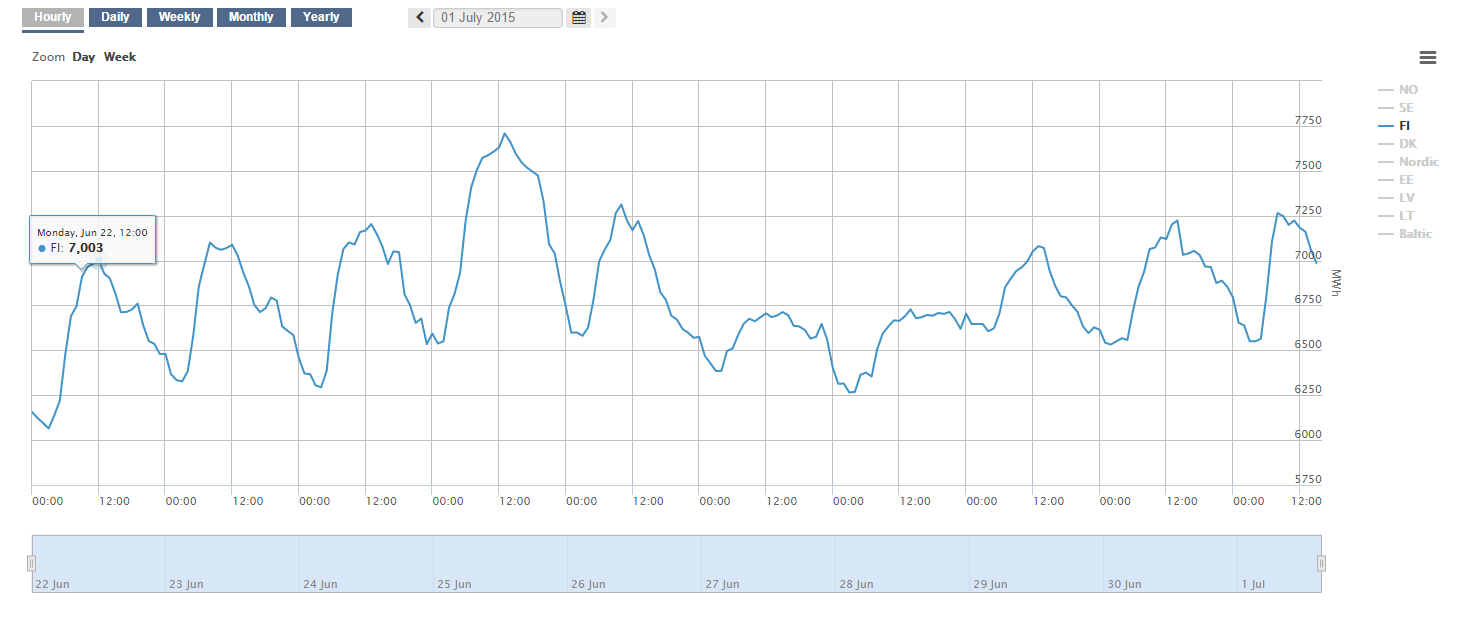
\includegraphics[width=1.00\textwidth]{figures/methodology/hourly_prices_finland.PNG}
	\caption{Finland hourly prices}
	\label{fig:hourly_prices_finland}
\end{figure}

\begin{figure}[!h]
	\centering
		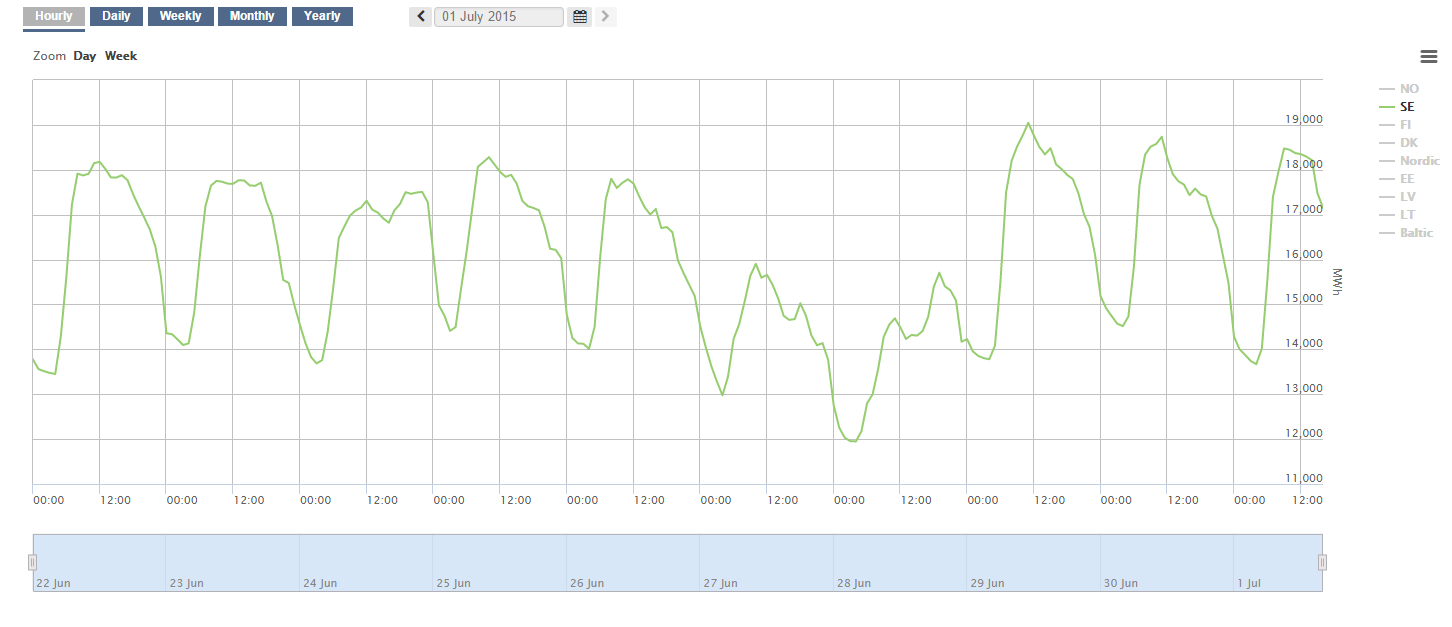
\includegraphics[width=1.00\textwidth]{figures/methodology/hourly_prices_sweden.PNG}
	\caption{Sweden hourly prices}
	\label{fig:hourly_prices_sweden}
\end{figure}




%
%
%[c BEGIN]
%
%\begin{itemize}[-]
%
%\item Financial market (Nasdaq OMX)
%Used for managing risks. Cash settled futures,
%forwards and options. Contracts can be made for
%up to six years. The system price is used as
%reference price.
%
%\item Day-ahead market (Nord Pool Spot)
%Day-ahead auction of power for delivery the next
%day. Nord Pool Spot calculates power prices
%based on supply and demand for every hour the
%following day.
%
%\item Intraday market (Nord Pool Spot)
%Continuous trading up to 30 minutes before
%delivery to adjust power production or
%consumption plans.
%
%\item Balancing market (TSOs)
%Operated by the respective transmission system
%operators. Final adjustments are made to ensure
%the correct frequency in the grid and security of
%supply
%
%\end{itemize}
%
%\emph{The future is Europe}
%
%The future of power trading lies in the
%creation of a single, integrated
%European market and an integrated
%platform.
%This will be the most advanced power
%market yet, offering efficiency in:
%
%\begin{itemize}
%\item Membership
%\item Management of collateral
%\item Cost
%\end{itemize}
%
%[c END] - Nord Pool Spot - Europe's leading power market \url{http://www.nordpoolspot.com/globalassets/download-center/annual-report/nord-pool-spot_europes-leading-power-markets.pdf}




%Nord Pool Spot - Day ahead market
%
%[c BEGIN]
%
%The day-ahead market, Elspot , is the main arena for trading power in the Nordic and Baltic region. Here, contracts are made between seller and buyer for the delivery of power the following day, the price is set and the trade is agreed.
%
%Today there are around 360 buyers and sellers (called members) on Elspot. Most of them trade every day, placing a total of around 2000 orders for power contracts on a daily basis.
%
%\emph{Driven by planning}
%
%Daily trading is driven by the members’ planning. A buyer, typically a utility, needs to assess how much energy (‘volume’) it will need to meet demand the following day, and how much it is willing to pay for this volume, hour by hour. The seller, for example the owner of a hydroelectric power plant, needs to decide how much he can deliver and at what price, hour by hour. These needs are reflected through orders entered by buyers and sellers into the Elspot trading system.
%
%\emph{Setting the price and closing the deal}
%
%12:00 CET is the deadline for submitting bids for power which will be delivered the following day. Elspot feeds the information into a specialist computer system which calculates the price, based on an advanced algorithm. Put simply, the price is set where the curves for sell price and buy price meet.
%
%\emph{Supply and demand}
%
%Hourly prices are typically announced to the market at 12:42 CET or later. Once the market prices have been calculated, trades are settled. From 00:00 CET the next day, power contracts are physically delivered (meaning that the power is provided to the buyer) hour for hour according to the contracts agreed.
%
%\emph{The cost of transmission constraints}
%
%While supply and demand are the key factors determining the hourly market prices, transmission capacity also plays a role. Bottlenecks can occur where power connections are linked to each other, if large volumes need to be transmitted to meet demand. To relieve this congestion, different area prices are introduced. In other words, when transmission capacity gets constrained, the price is raised to reduce demand in the areas affected.
%
%[c END] - Nord pool Spot Elspot Market \url{http://www.nordpoolspot.com/How-does-it-work/Day-ahead-market-Elspot-/}



%Nord Pool Spot - Intraday market
%
%[c BEGIN]
%
%Elbas  is an intraday market for trading power operated by Nord Pool Spot. Covering the Nordic and Baltic region as well as Germany and recently extended to include the UK, Elbas supplements Elspot and helps secure the necessary balance between supply and demand in the power market for Northern Europe.
%
%The majority of the volume handled by Nord Pool Spot is traded on the day-ahead market. For the most part, the balance between supply and demand is secured here. However, incidents may take place between the closing of Elspot at noon CET and delivery the next day. A nuclear power plant may stop operating in Sweden, or strong winds may cause higher power generation than planned at wind turbine plants in Germany. At Elbas, buyers and sellers can trade volumes close to real time to bring the market back in balance.
%
%Trading close to real time
%
%At 14:00 CET, capacities available for Elbas trading are published. Elbas is a continuous market, and trading takes place every day around the clock until one hour before delivery. Prices are set based on a first-come, first-served principle, where best prices come first – highest buy price and lowest sell price.
%
%Increasingly important
%
%The intraday market is becoming increasingly important as more wind power enters the grid. Wind power is unpredictable by nature, and imbalances between day-ahead contracts and produced volume often need to be offset. Elbas will play a key role in the development of intraday power trading in Europe. Future prospects indicate exponential growth, reaching 1.900 GW installed wind capacity worldwide in 2020 (Source: World Wind Energy Association). This type of market can be a key enabler to increase the share of renewable energy in the energy mix. 
%
%[c END] - Nord pool Spot Intraday Market \url{http://www.nordpoolspot.com/How-does-it-work/Intraday-market/}




\subsubsection{ISO New England}

The market of ISO New England offers day ahead as well as real time energy prices where day ahead prices are available at an hourly interval while (preliminary) real time prices are available both at hourly and five minute intervals\footnote{\url{http://www.iso-ne.com/}}. 

Current locational marginal prices (LMPs) can be downloaded from a base url\footnote{\url{http://www.iso-ne.com/static-transform/csv/histRpts/da-lmp/}} and a specialized suffix depending on the file and date (e.g.~WW\_DALMP\_ISO\_20150414.csv). In this case, files are provided in csv format for better machine processing. 

%Example: 
%\begin{verbatim}
	%H,"Date","Hour Ending","Location ID","Location Name","Location Type","Locational Marginal Price",
	%"Energy Component","Congestion Component","Marginal Loss Component"
	%D,"04/14/2015","02","4006",".Z.SEMASS","LOAD ZONE",14.82,14.85,0.01,-0.04
	%D,"04/14/2015","02","4007",".Z.WCMASS","LOAD ZONE",14.94,14.85,0.01,0.08
	%D,"04/14/2015","02","4008",".Z.NEMASSBOST","LOAD ZONE",14.84,14.85,0.01,-0.02
%\end{verbatim}

A summary of all data that is available is provided for day ahead as well as real time prices\footnote{\url{http://www.iso-ne.com/isoexpress/web/reports/pricing/-/tree/zone-info}}. It is described as ``zonal information'' on the website to emphasize the locational character of the prices. 


\subsubsection{EEX}

The European Energy Exchange (EEX) is a power market operating for the market area of France, Germany/Austria and Switzerland. Each of these regions exhibits a separate spot market where prices are traded for the respective country. 
The actual trading takes place on EPEX SPOT, an organisation that drives the integration of power markets in Europe where EEX is a part of. It consists of an intraday (real time) and day ahead market for trading during the day and for the next day, respectively. 

Several info products are available on the market for end-of-day data (EOD) that cover historical as well as current trading data from the spot and derivatives markets. 
Data is available on subscription for all of the above mentioned regions. Available data formats include csv, excel and xml files, provided on demand on a ftp server. 
Depending on the type of product and the time period available different fees apply and have to be paid in advance. 
Access is granted to a vast amount of historical energy price data for the derivatives as well as the spot market for energy and other commodities like natural gas and coal where both prices and trading volumes are included. 

Naming conventions designating the different areas of trading are defined as follows: 

\begin{itemize}

\item \emph{PHELIX} The Physical Electricity Index denotes the area of Germany and Austria

\item \emph{SWISSIX} The Swiss Index denotes the area of Switzerland

\item \emph{FRANCE} The index for France denotes the area of France

\item \emph{ELIX} The European Electricity Index defines prices valid for all of Europe (?)

\end{itemize}


\subsubsection{APG}

Austrian Power Grid\footnote{\url{http://www.apg.at/de/markt/strommarkt}}



\subsubsection{PJM}

See at \url{http://www.pjm.com/}. 


\subsubsection{OMIE - Spanish power market}

OMIE represents the wholesale energy market for the iberian region. \footnote{\url{http://www.omel.com/en/inicio}}

EDP (Energias de Portugal) is an energy company in cooperation with the wholesale electricity market for Spain, Portugal and is also responsible for delivery and transmission of energy to other countries. \footnote{\url{http://www.edp.pt/en/aedp/sectordeenergia/sistemaelectricoespanhol/Pages/SistElectES.aspx}}


\subsubsection{Brazilian power market}

The brazilian power market exhibits special conditions as it is heavily based on hydro power generation \cite{reston2012short}. In this market the tight pool model is applied where generation dispatch is centralized by an Independent System Operator (ISO). 



\subsection{Terms and definitions}

\subsubsection{Definition of 'Clearing Price'}

The following is a definition of clearing price from Investopedia\footnote{\url{http://www.investopedia.com/terms/c/clearingprice.asp}}. 

\begin{quote}
The specified monetary value assigned to a security or asset. This price is determined by the bid and ask process of buyers and sellers interested in trading the security.

In any exchange, sellers prefer to part with their assets for the highest price possible while investors interested in buying the same asset desire the lowest purchase price possible. At some point, a mutually agreeable price is reached between buyers and sellers. It is at this point that economists say the market has "cleared" and transactions take place. Thus, the clearing price of an asset is the price at which it was most recently traded.
\end{quote}



%google Search : "`tight pool models electricity"'
%
%Google Books "`Making Competition Work in Electricity"'
%\url{https://books.google.at/books?id=Pki4tu3P8iIC&pg=PA286\&lpg=PA286\&dq=tight+pool+models+electricity\&source=bl\&ots=drkU0A9H3C\&sig=m_J7JCkGjf5ydml2fdbFQB50ojE\&hl=de\&sa=X\&ved=0CCQQ6AEwAGoVChMIgoLZjffmxgIVTLYUCh3DEQBT#v=onepage\&q=tight\%20pool\%20models\%20electricity\&f=false}
%
%Also see Figure 3.2 in the book on page 43. 
%
%Chapter 4: Requirements for competition- Demand side

The clearing price is set at the intersection of the demand and supply curves, see Figure \ref{fig:market_demand_supply}



\begin{figure}[!h]
	\centering
		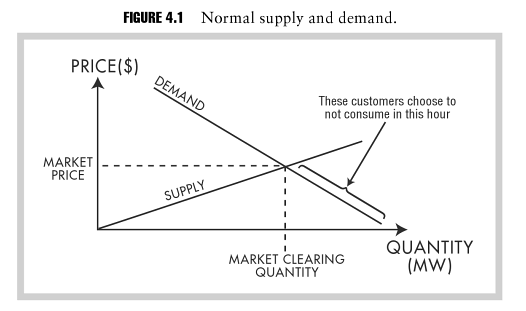
\includegraphics{figures/methodology/market_demand_supply.PNG}
	\caption{Demand Supply Chart}
	\label{fig:market_demand_supply}
\end{figure}



\subsubsection{Locational marginal price}

See definition by ISO-NE\footnote{\url{http://www.iso-ne.com/participate/support/faq/lmp}}. 

%TODO explain LMP (-> see ISO New England energy data, \textbf{smd hourly}!)

\subsubsection{System marginal price (SMP)}

A price type described by \cite{szkuta1999electricity}. 

\subsubsection{System Load}

%TODO

Some energy markets provide the total system load as measured by metering. It is used for day-ahead and long term forecasting purposes and in addition it serves as important indicator in reports. The system load for the ISO New England energy market is calculated by $System Load = generation - pumping + net\_interchange$


\subsubsection{Forward Capacity Market (FCM)} 

A forward capacity market is used to ensure having enough capacity for a specific amount of time into the future. A capacity commitment period (CCP) ensures that a certain amount of capacity will be available during that period. For example, the CCP at ISO-NE is set as one year ranging from June 1st until May 31st. 

The market has to ensure that the \emph{Installed Capacity Requirements (ICR)} for the corresponding region are met. These requirements are defined for each capacity commitment period and define the amount of capacity needed to meet estimated peak and reserve demands. Important measures to define the ICR are the local sourcing requirements (LSR) and maximum capacity limits (MCL) that define the constraints given by market participants. %(QUOTE)In addition the Hydro-Québec Interconnection Capability Credits (HQICCs), are a key input into the calculation of the ICR.

The actual procurement of resources for each capacity commitment period is determined by a \emph{Forward Capacity Auction (FCA)} which aims to meet the defined ICRs for the given period.
This auction is carried out three years ahead of the related CCP to ensure that enough resources will be available during that period. \emph{Reconfiguration Auctions (RA)} are then executed annually until the start of the CCP and continued monthly afterward. During an RA capacity resources may be amended to adapt to potential changes in capacity zones. 

At the FCM of ISO New England there is also the option of making a composite offer where different capacity resources may join their capacity offers (useful i.e.~in case of single season capacities) to result in a single resource offer at the market. 

%Capacity resources <-> energy suppliers/providers?

%See definition at the website of ISO NE\footnote{\url{http://www.iso-ne.com/markets-operations/markets/forward-capacity-market}}.

\subsubsection{Regulation market}

Definition by the ISO NE power market\footnote{\url{http://www.iso-ne.com/markets-operations/markets/regulation-market}}:

\begin{quote}
The Regulation Market is the mechanism for selecting and compensating market participants to provide regulation—the capability of specially equipped generators and other energy sources to increase or decrease output or consumption every four seconds. Participants allow their Automatic Generation Control (AGC) resources to be controlled by the ISO using automated signals to balance both second-by-second variations in demand and the system frequency, which must be kept constant. This market helps ensure that the ISO meets the North American Electric Reliability Corporation Real Power Balancing Control Performance Standard (BAL-001-0). Two regulation clearing prices are calculated: one for capacity and one for actual service mileage.
\end{quote}




\subsubsection{Two settlement system: Day ahead vs Balancing market}

A two settlement system has been defined for the PJM power market (PJM standing for Pennsylvania, Jersey, Maryland)\cite{lambert2001creating}. 

A two-settlement system in power markets is understood as a system comprising a day ahead as well as a real time (balancing) power market\cite{lambert2001creating}. 




\section{Forecasting}

\subsection{Introduction}

Since the occurrence of competitive energy markets forecasting of energy prices has been vital to utility operators. 


\subsection{Forecasting models}

%TODO
Discussion of suitable models for price time series from various energy markets. 


\subsubsection{Random walk}

A random walk model is best suited for series that exhibit major fluctuations on a short term and where no apparent trend can be recognized \cite{makridakisforecasting}(pg. 461). Thus this model can be described by an accumulation of a random error over time (equation \ref{eq:random_walk}). 

\begin{equation}
Y_t = \sum e_t
\label{eq:random_walk}
\end{equation}

$Y_t$ denotes the value of the time series at time point $t$ whereas $e_t$ is a timeseries of random errors where the errors exhibit no correlation and are normally distributed \cite{makridakisforecasting}(pg. 461). 

In \cite{makridakisforecasting}(pg. 464) it is stated that the behavior of economic and business series in particular can be characterized by a random walk model since they show so-called cycles or random fluctuations around a possible trend. 

As it is impossible to accurately predict upcoming values or cycles of a random walk model by definition one of the most suitable prediction models is the ``naive forecast'' where the forecasted value of the upcoming timestamp is set equal to the last observed value (equation \ref{eq:naive_forecast}).

\begin{equation}
\hat{Y}_{t+i} = Y_t
\label{eq:naive_forecast}
\end{equation}



\subsubsection{ARIMA models}

\emph{ARIMA model generation}

See Box-Jenkins Methodology. 


\subsubsection{Neural Network models}

An approach of using artificial neural networks (ANN) as a model to forecast short term electricity prices is presented in \cite{szkuta1999electricity}. 


\paragraph{Competition}

Neural network forecasting competition available from 2008\footnote{\url{http://www.neural-forecasting-competition.com/NN5/}}. 




\subsubsection{Forecasting benchmarks}






\subsection{Accuracy measures}


\subsection{Model selection}



\subsubsection{Autocorrelation}



The autocorrelation function determines the existence or non-existence of correlation between lagged variables within a time series. 

That is, the correlation between a point in the time series to another point in the same time series is calculated where the gap between the two points is fixed by the given lag. 

The autocorrelation is calculated as an autocorrelation coefficient in equation \ref{eq:autocorr_coeff}

\begin{equation}
R_h = \frac{C_h}{C_0}
\label{eq:autocorr_coeff}
\end{equation}


where $C_h$ denotes the autocovariance function and $C_0$ the variance function 
(see equations \ref{eq:autocov_func} and \ref{eq:variance_func}). 


\begin{equation}
C_h = \frac{1}{N} \sum\limits_{t=1}^{N-h} (Y_t - \bar{Y}) (Y_{t+h} - \bar{Y})
\label{eq:autocov_func}
\end{equation}


\begin{equation}
C_0 = \frac{1}{N} \sum\limits_{t=1}^{N} (Y_t - \bar{Y})^2
\label{eq:variance_func}
\end{equation}


Explanation: The autocovariance function determines the (average) covariance between variables with the given lag while the variance function determines the maximum (average) variance over all timestamps (t=1 to N). 


See \url{http://www.itl.nist.gov/div898/handbook/eda/section3/autocopl.htm}


\subsubsection{Box Cox transformation}

The Box Cox transformation is used to transform a series based on a non-normal distribution to a normal distribution. This is done via log and exponential transformations. 

See \url{http://www.isixsigma.com/tools-templates/normality/making-data-normal-using-box-cox-power-transformation/}



\subsection{Energy price related forecasts}



\section{Cloud-based Simulator}


\subsection{Motivation}

\subsection{Structure of simulator}

\subsection{Functional requirements}

%TODO 
Discuss impact of evaluation of bandwidth costs. In \cite{rao2010minimizing} %(page 7) 
bandwidth costs are deliberately neglected, but the option should be still taken into account. As these costs directly relate to costs of migrations it is vital to include and model them within the scenarios. 

\subsection{Non-functional requirements}

\subsection{Incorporating forecast models}

As already discussed in the introduction %TODO WHERE ?(forecast chapter? TODO) 
forecasting is an integral component of the simulation as it should support in decision making when assigning workload and performing migrations. Since forecast errors can have a negative impact on workload allocation which may result in non-optimal workload distributions \cite{de2013study} it is of paramount importance that the forecast models are trained thoroughly and forecast errors are kept at a minimum. In order to reduce the impact of forecast errors in the simulation forecasting is done several hours into the future whereby the results are averaged to obtain a broader estimate of energy prices of the near future. 


\subsection{Simulation runs}



\section{Cost models}

Cost models are required to map the servers' energy consumption to costs depending on current energy prices. Different cost models exist exhibiting higher or lower accuracy and differ in their type of calculation. 

In this thesis several assumptions have been made: 

\begin{itemize}

\item \textbf{idle power.} A server has a defined idle power (e.g.~100 Watts (W)). This is the power that is drawn when the server is in idle mode (no tasks are running). 

\item \textbf{peak power.} A server has a defined peak power (e.g.~200 Watts (W)). This is the power that is drawn when the server runs on maximum load (maximum number of tasks running). 

\item \textbf{utilization.} Each server has a utilization between 0 and 100 percent. A utilization of zero percent means the server is idle, in contrast a utilization of hundred percent means the server is at peak load. 

\item \textbf{power consumption.} The power consumption is defined as the effective power consumed by a server during a certain period of time (e.g.~one hour). The result is a measure of power consumed per time (e.g.~150 Watt hours (Wh) for a server running on 50\% utilization for one hour)\footnote{\url{http://whatis.techtarget.com/definition/kilowatt-hour-kWh}}. %Energy can also be measured in Joule (J) where one Watt (W) equals 1 Joule per second (J/s)\footnote{\url{http://en.wikipedia.org/wiki/Kilowatt_hour}}. Thus one kilowatt hour equals $3.6 * 10^6$ kilojoules. 

\item \textbf{energy price.} The energy price is taken from the energy market that the data center is connected to. These prices typically change every hour which is therefore the relevant time interval for all further operations. 

\end{itemize}

From these assumptions a simple cost model can be derived. Since power is measured per hour in Watts and prices are given per Kilowatt Hours (kWh) the power consumed by servers can be directly mapped to energy costs. This model is simplified in that it does not consider frequency scaling or other power measures taken for a server (suspend, sleep mode). Thus it serves as a base for comparing different scenarios and it is also useful to get a first impression on the overall power consumption and costs involved in a given scenario. 

A cost model is essential for evaluating the usefulness of the approach presented in this thesis as the ultimate goal is to reduce energy related costs of geographically distributed and connected data centers based on changing energy prices. 





%%%%%%%%%%%%%%%%%%%%%%%%%%%%%%%%%%%%%%%%%
\chapter{Results}
\label{ch:results}
%%%%%%%%%%%%%%%%%%%%%%%%%%%%%%%%%%%%%%%%%



\section{Architectural outline}

%\subsection{Application Server}
%
%\subsubsection{Datamanagement}
%
%\subsubsection{Web Services}
%
%\subsubsection{Scheduling}
%
%
%\subsection{R Server}
%
%\subsubsection{Forecast Models}
%
%\subsubsection{Assessment of Forecasts}
%
%\subsubsection{Forecast error evaluation}
%
%
%\subsection{Simulator}
%
%\subsubsection{Basic structure}
%
%\subsubsection{Configuration}
%
%\subsubsection{External interfaces}
%
%\subsubsection{Scheduler}




% Scheduler Types

% Benefits and drawbacks
 
% Settings and configuration



\section{Model selection}


\section{Simulation and Scheduling}


\section{Statistics and Empirical Evaluation}




%%%%%%%%%%%%%%%%%%%%%%%%%%%%%%%%%%%%%%%%%
\chapter{Discussion}
\label{ch:discussion}
%%%%%%%%%%%%%%%%%%%%%%%%%%%%%%%%%%%%%%%%%



\section{Benefits and limitations}



...

As Qureshi et al.~pointed out in \cite{qureshi2009cutting} most companies would need to renegotiate their energy contracts in order to utilize the proposed approach. Companies renting space in co-location facilities usually pay a fixed price for energy rather than directly taking part in the price offers of wholesale markets. 

Demand response programs are a way of further decreasing energy costs as consumers agree on a reduced price in exchange for a reduced load when it is requested by the grid operator\cite{albadi2008summary}. This is certainly interesting for energy elastic distributed systems that are able to shift load to other locations dynamically. 



\section{Comparison of Related Work}


\section{Discussion of open issues}

%%%%%%%%%%%%%%%%%%%%%%%%%%%%%%%%%%%%%%%%%
\chapter{Conclusion}
\label{ch:conclusion}
%%%%%%%%%%%%%%%%%%%%%%%%%%%%%%%%%%%%%%%%%






ARIMA models showed reasonably good performance, in many cases they showed the best results compared to other evaluated models in this work. 







In \cite{de2013study} it is shown that the cost of optimal assignment is further reduced by increasing the number of locations with data centers assigned to different energy markets and/or by increasing the variability of energy prices. 


\section{Benefits and limitations}



...

As Qureshi et al.~pointed out in \cite{qureshi2009cutting} most companies would need to renegotiate their energy contracts in order to utilize the proposed approach. Companies renting space in co-location facilities usually pay a fixed price for energy rather than directly taking part in the price offers of wholesale markets. 

Demand response programs are a way of further decreasing energy costs as consumers agree on a reduced price in exchange for a reduced load when it is requested by the grid operator\cite{albadi2008summary}. This is certainly interesting for energy elastic distributed systems that are able to shift load to other locations dynamically. 






\section{Future Work}


Forecasting models may be improved, or different models may be investigated based on electricity price data. 

Dynamic Regression (DR) and Transfer function (TF) models have been shown to provide a significantly better performance than ARIMA models \cite{aggarwal2009electricity,weron2005forecasting}. This may be due to the additional regressor variables that are considered in multivariate models (DR and TF) in contrast to models based on a single univariate time series (ARIMA). 

In general multivariate models seem to provide better results than univariate models as they are able to include more information into the model generation process \cite{weron2005forecasting}. 


%%%%%%%%%%%%%%%%%%%%%%%%%%%%%%%%%%%%%%%%%
%%% BACKMATTER %%%%%%%%%%%%%%%%%%%%%%%%%%
%%%%%%%%%%%%%%%%%%%%%%%%%%%%%%%%%%%%%%%%%

\appendix

\bibliographystyle{plain}
\bibliography{references}

\end{document}
